% \section{MHLC Task and MatchIntel2 Benchmark} 
% \begin{figure*}[t]
%     \centering
%     \fbox{
%         \parbox{0.95\textwidth}{
%         \textbf{Pipeline Figure Placeholder (to be replaced).}
%         Suggested layout: left-to-right, 4 blocks.\\
%         Block A (Input): Numerical sequences + player heatmaps (non-semantic observations).\\
%         Block B (Task Core): Understanding $\rightarrow$ Synthesis $\rightarrow$ Reasoning (MHLC core process).\\
%         Block C (Modeling Paths): (i) General LMs / PEFT; (ii) Specialized lightweight models.\\
%         Block D (Evaluation): MCQ / SCQ / TFQ + random-level threshold comparison.\\
%         Add two highlight arrows: ``semantic shortcut removed'' and ``cognitive collapse vs specialized success''.
%         }
%     }
%     \caption{Design placeholder for the full MHLC pipeline figure in Section~\ref{sec:mhlc-benchmark}.}
%     \label{fig:pipeline_placeholder}
% \end{figure*}


% \begin{figure}[t!]
% 	\centering
% 	
\includegraphics[scale=0.10]{pic2.pdf}
% 	\caption{An illustration of our work.}
% 	\label{figure1}
% \end{figure}

% \begin{figure}[t] % [t] 表示放在页面顶部，顶会常用
%     \centering
%     % 第一张子图
%     \begin{subfigure}[b]{0.48\textwidth}
%         \centering
%         
\includegraphics[width=\textwidth]{pic3.pdf}
%         \caption{Numerical Modality: real-time statistical numerical sequences.}
%         \label{fig:pic3}
%     \end{subfigure}
%     \begin{subfigure}[b]{0.48\textwidth}
%         \centering
%         
\includegraphics[width=\textwidth]{pic5.pdf}
%         \caption{Visual Modality: player position visual heatmaps.} 
%         \label{fig:pic4}
%     \end{subfigure}
%     \caption{An example of input data in the dataset.}
%     \label{fig5}
% \end{figure}

% \begin{figure}
% 	\centering
% 	
\includegraphics[scale=0.22]{pic3.pdf}
% 	\hfil
%         
\includegraphics[scale=0.185]{pic4.pdf}
% 	\caption{Principle of single-step sampling.}
% 	\label{fig5}
% \end{figure}



% \subsection{Problem Formulation of MHLC}
% The MHLC task examines whether models can derive high-level conclusions from fragmented non-semantic observations across modalities. Specifically, the inputs are low-level numerical sequences and visual spatial topologies, while the outputs are high-level tactical style labels. Solving this task requires the integration of understanding, synthesis, and reasoning, rather than direct semantic matching or low-level signal extrapolation.

% Compared with conventional multimodal tasks, MHLC emphasizes inference over latent physical-world logic. The key challenge lies in the fact that neither an individual numerical value nor a single heatmap region can directly determine the final conclusion; models must construct an implicit global representation from fragmented evidence before making decisions.

% To make this requirement explicit, we decompose MHLC into three consecutive cognitive capabilities operating on non-semantic observations:
% \begin{itemize}
%     \item \textbf{Understanding (U):} interpret fragmented numerical statistics and spatial topologies into latent local evidence states.
%     \item \textbf{Synthesising (S):} integrate local evidence across time/space into an implicit global framework of the match.
%     \item \textbf{Reasoning (R):} map the global framework to high-level tactical style labels.
% \end{itemize}

% Under this formulation, success is not simply entity matching (e.g., “what label name looks similar”) nor low-level prediction, but requires consistent U $\rightarrow$ S $\rightarrow$ R cognition even when semantic entities are absent.

% Formally, each sample is denoted as $\mathcal{X}=(\mathcal{X}^{num}, \mathcal{X}^{vis})$, where $\mathcal{X}^{num}$ denotes real-time statistical numerical sequences and $\mathcal{X}^{vis}$ denotes a set of player-position heatmaps. The prediction target is a multi-label vector $\mathbf{y}\in\{0,1\}^{K}$ over a finite style set $\mathcal{Y}$. The MHLC objective is to learn a mapping
% \[
% f_{\theta}: (\mathcal{X}^{num}, \mathcal{X}^{vis}) \rightarrow \mathbf{y},
% \]
% such that high-level style conclusions are inferred from low-level, fragmented, and non-semantic observations.

% To align with prior HLC work and enable strict comparability, we instantiate evaluation with three QA-style formats (MCQ/SCQ/TFQ) that share the same label semantics while probing different decision granularities: selecting one label (SCQ), selecting multiple labels (MCQ), and judging a candidate label set (TFQ). Therefore, improvements must come from better perception and integration of non-semantic evidence, rather than from format-specific heuristics.

% \subsection{Benchmark Construction}
% Existing multimodal datasets are mostly confined to low-level mechanical processing, where low-level inputs are transformed into low-level outputs. Such settings are insufficient for evaluating whether models can obtain high-level conclusions by perceiving latent physical-world logic. To bridge this gap, we construct a new benchmark from WhoScored, a professional football analysis website widely used in sports analytics.

% The benchmark construction includes two components:
% \begin{itemize}
%     \item \textbf{Low-level input.} Fine-grained statistical data at each time step are extracted from Match Centre, covering cumulative features from fundamental actions (e.g., passes, dribbles) to situational events (e.g., zones, direction). In parallel, visual positional heatmaps of participating players across the full match are collected. The raw nature of these observations makes the inputs low-level and fragmented.
%     \item \textbf{High-level output.} Team-style summaries are extracted from Match Report and normalized into a finite label set of 12 playing styles: \textit{Played with width; Favoured long shots; Favoured short passing; Attacked through the middle; Favoured through balls; Attacked down the left side; Favoured crossing the ball; Favoured long balls; Had a high shot frequency when in possession; Dominated possession; Attacked down the right side; Had a large quantity of possession in their opponent's half}. These labels cannot be determined from isolated observations and require integrated understanding, synthesis, and reasoning, so they serve as high-level conclusions.
% \end{itemize}

% All collected samples are compiled into a standardized JSON format for subsequent training and evaluation.


% \begin{itemize}
%  % 分两列显示，节省空间
%     \item \textit{Played with width}
%     \item \textit{Favoured long shots}
%     \item \textit{Favoured short passing}
%     \item \textit{Attacked through the middle}
%     \item \textit{Favoured through balls}
%     \item \textit{Attacked down the left side}
%     \item \textit{Favoured crossing the ball}
%     \item \textit{Favoured long balls}
%     \item \textit{Had a high shot frequency when in possession}
%     \item \textit{Dominated possession}
%     \item \textit{Attacked down the right side}
%     \item \textit{Had a large quantity of possession in their opponent's half}
%         % ... 在这里补全12个
% \end{itemize}

% \subsection{Evaluation Protocol}
% To maintain consistency with prior HLC evaluation, we follow Liu et al. \cite{liu2025can} and instantiate three assessment formats:
% \begin{itemize}
%     \item \textbf{MCQ:} extract two to four appropriate playing styles from four candidates.
%     \item \textbf{SCQ:} select one correct playing style from four candidates.
%     \item \textbf{TFQ:} judge whether a presented style set is absolutely correct.
% \end{itemize}

% For direct comparability with textual-modality evaluation, instruction semantics are kept aligned, while commentary text is replaced by numerical or visual inputs. We then extract predicted styles from model outputs. Any content outside the finite label set is treated as invalid, since failure to follow the answer space indicates weakness in task-level understanding. Lightweight models output multi-label probabilities directly, and all models are scored by matching predictions with ground truth labels.

% To define a strict cognitive boundary, we use a mathematical random-level baseline for all three formats. Based on combinatorial probability, expected random accuracies ($P$) are $1/2$ for TFQ, $1/4$ for SCQ, and $1/11$ for MCQ. To reduce random-chance effects, we adopt the upper bound of the 99.7\% confidence interval, i.e., $P+3\sigma$ where $\sigma=\sqrt{P(1-P)/n}$. The resulting thresholds are 0.547 (TFQ), 0.291 (SCQ), and 0.118 (MCQ), which are used as criteria for exhibiting MHLC.



\section{GWC Framework} 

\label{sec:mhlc-benchmark}
% This section formalizes the MHLC task and introduces the MatchIntel2 benchmark. The presentation follows a direct logic: we first define the task, then describe benchmark construction, and finally specify the evaluation protocol used to test modality-agnostic high-level cognition.
\subsection{Problem Formulation of GWC}
Based on the three core characteristics of Gestalt World-Level Capability (GWC), we formalize its definition as follows:

1) Modality-Agnostic:Confronted with the complex, heterogeneous representations of the physical world, GWC relies on an underlying, ubiquitous processing mechanism. For any given modality $m \in \{\text{num}, \text{vis}, \text{text}, \dots\}$, the macroscopic Gestalt mechanism of GWC, denoted as $\mathcal{F}$, must satisfy Representational Equivalence. Specifically, when disparate modalities $m_a$ and $m_b$ observe the same objective physical event $\mathcal{E}$, this mechanism must transcend representational barriers to ensure absolute consistency in the derived conclusions, fundamentally eliminating reliance on modality-specific or explicit semantic shortcuts:$$\mathcal{F}(\mathcal{X}^{m_a}) \equiv \mathcal{F}(\mathcal{X}^{m_b}) \rightarrow \mathbf{y}_{\mathcal{E}}$$

2) High-Level Cognition:The essence of processing the complex physical world lies in bridging the representational chasm between low-level data and high-dimensional principles. Liu et al. [cite] define high-level cognition as the transitional process of deriving high-level conclusions from low-level and fragmented foundational information, instantiating it as an "Understanding-Synthesizing-Reasoning" chain structure ($f_R \circ f_S \circ f_U$). We introduce this paradigm to process heterogeneous physical observations $\mathcal{X}^{m}$:Understanding ($f_U$): Operates independently on each fragmented, low-level physical segment to extract isolated local features: $\mathcal{H}_{local}^{m} = \{ f_{U}(x_{i}^{m}) \}_{i=1}^{N_{m}}$.Synthesizing ($f_S$): Integrates all fragmented local features to construct a coherent, implicit global representation: $\mathbf{H}_{global}^{m} = f_{S}(\mathcal{H}_{local}^{m})$.Reasoning ($f_R$): Derives high-level conclusions regarding the physical world (e.g., high-dimensional intentions, macroscopic laws) based on this global representation: $\mathbf{y} = f_{R}(\mathbf{H}_{global}^{m})$.

3) Open-ended Evolution:Analogous to neuroplasticity in the human brain, the model must achieve continuous reshaping of its endogenous logic through dynamic interaction with the physical environment. This dynamic process exhibits an iterative, upward trajectory alongside the interaction step $t$:$$\theta^{(t+1)} = \theta^{(t)} + \Delta \theta \left( \mathcal{X}_{t}^{m}, \text{Feedback}_{t}, \mathcal{F}_{\theta^{(t)}} \right)$$This ensures the model can continuously shatter its inherent cognitive boundaries and seamlessly adapt to the open-ended, boundless, and complex evolution of the physical world.




\begin{figure*}[!t]
	\centering
	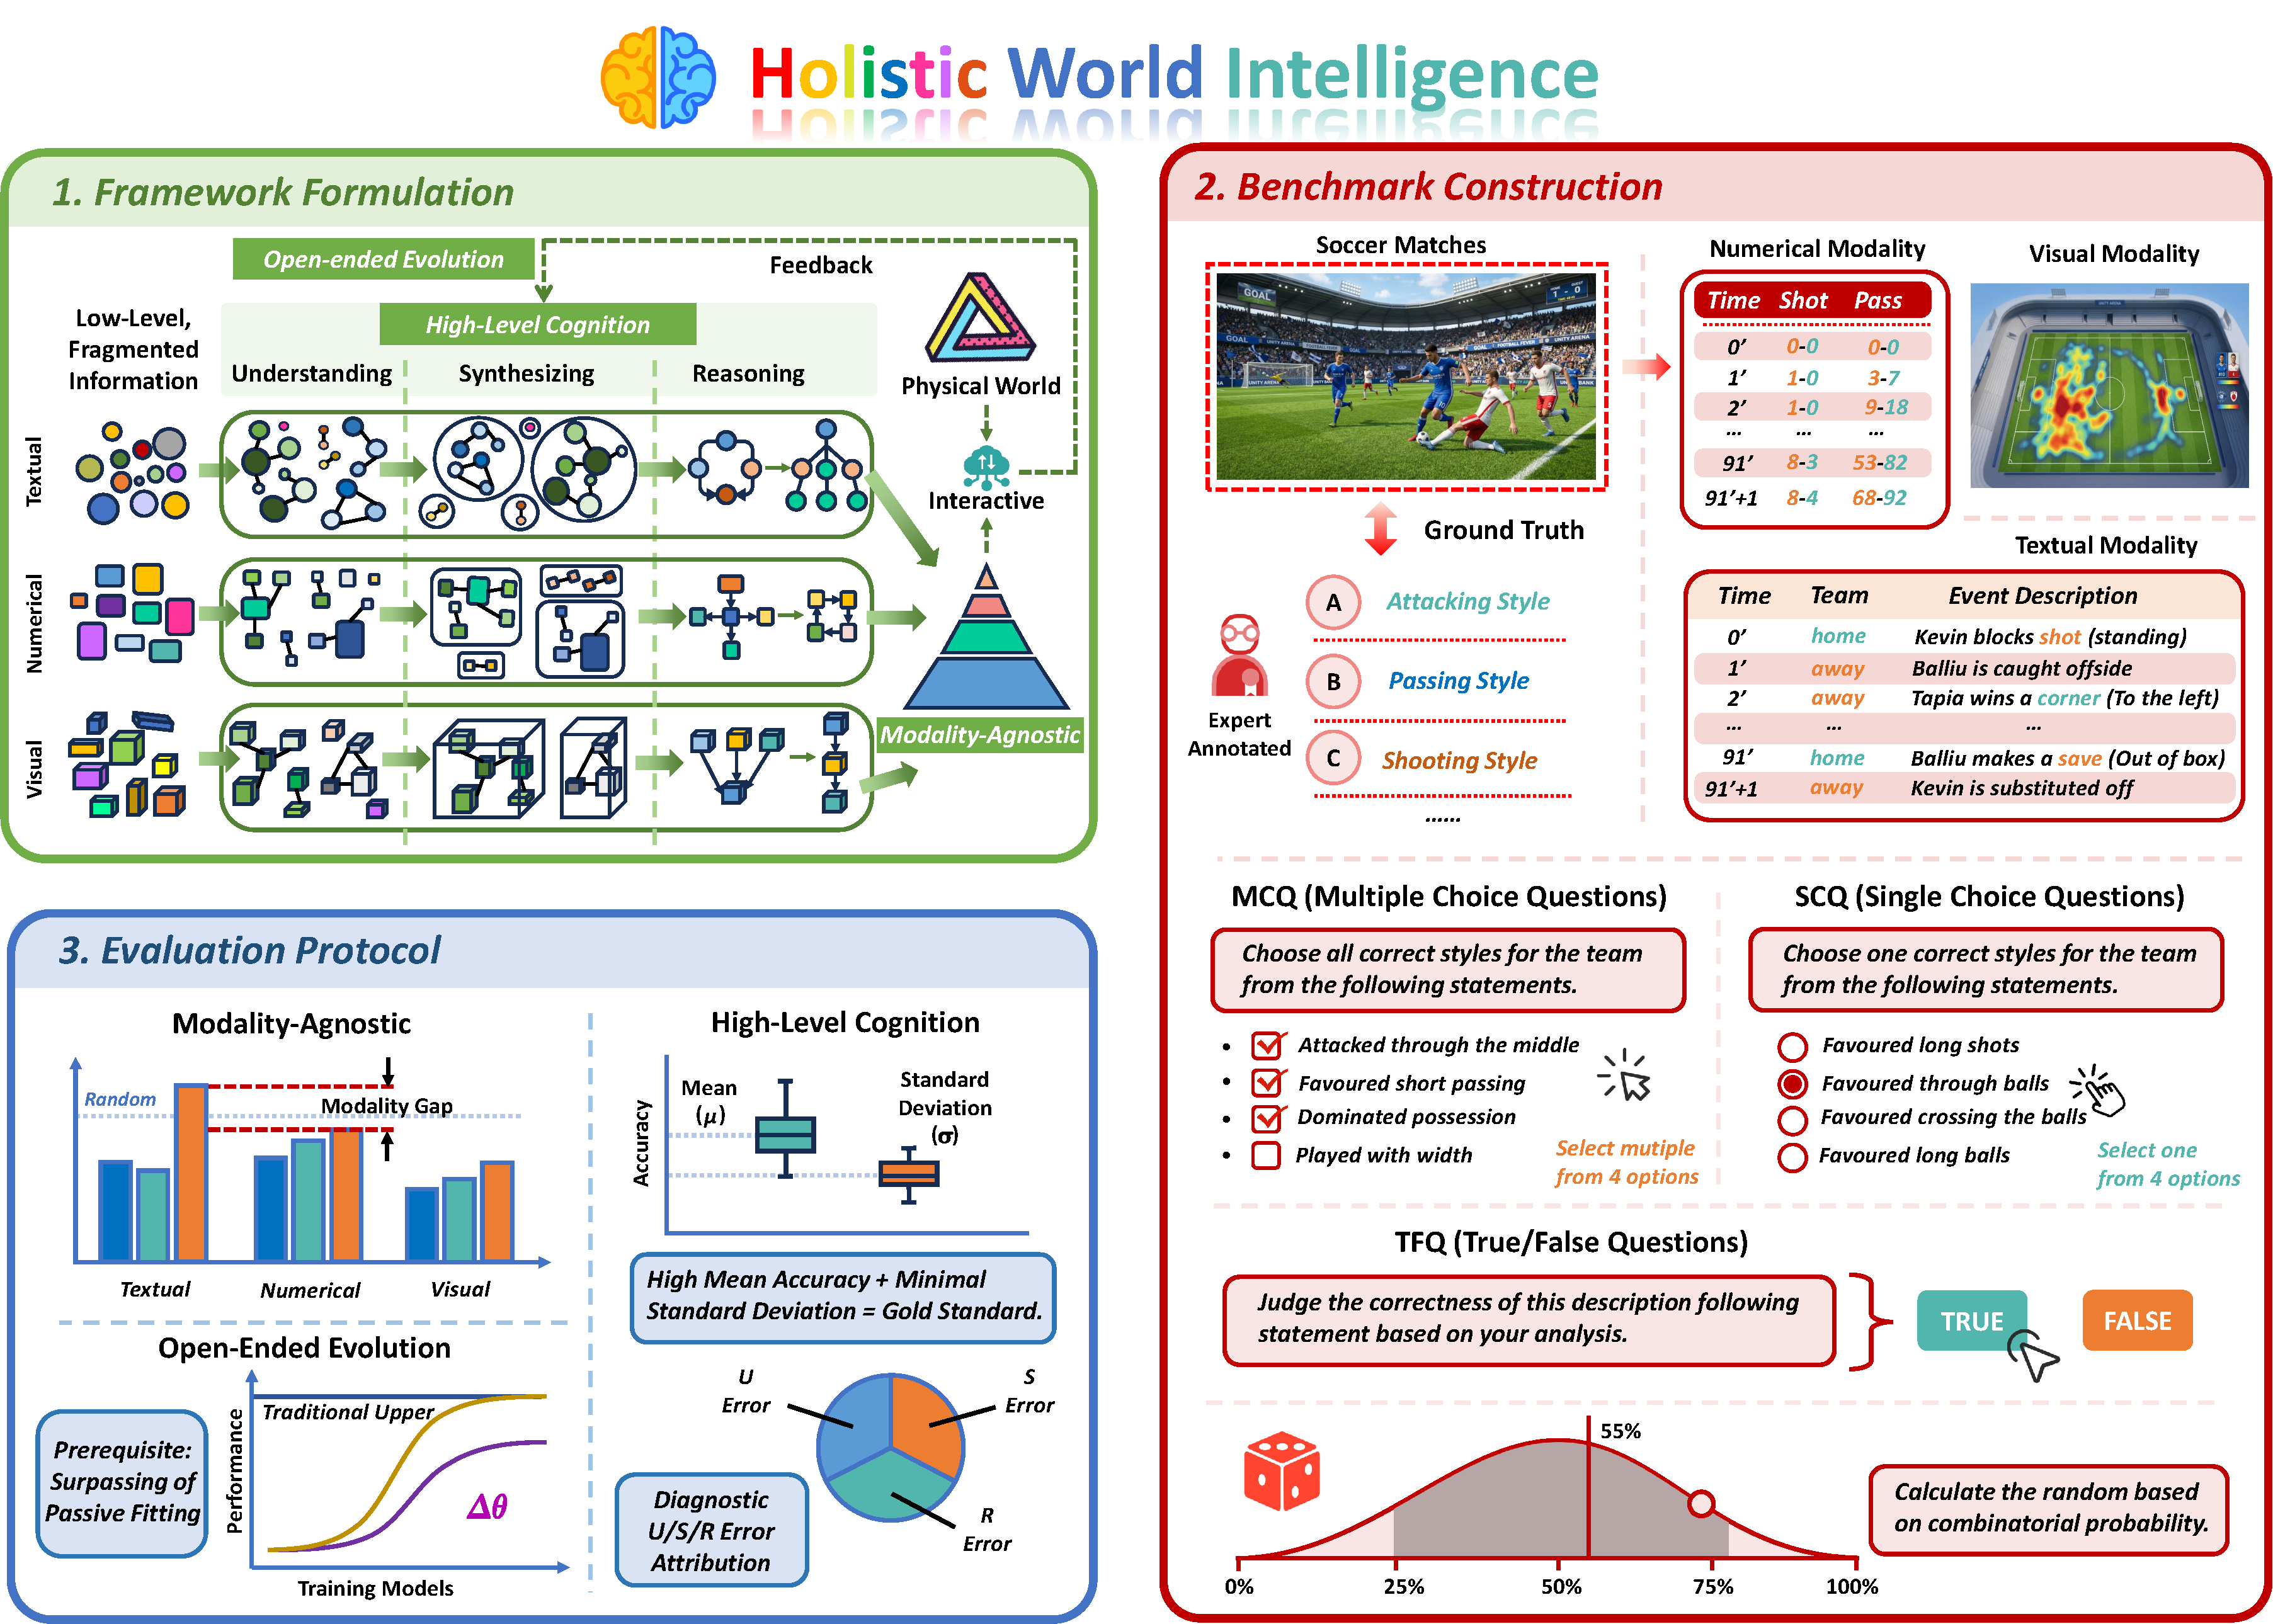
\includegraphics[scale=0.28]{figure/figure2.pdf}
	\caption{Pipeline Figure. }
	\label{figure1}
\end{figure*}

\subsection{Benchmark Construction}
\subsubsection{Data collection}
Existing datasets predominantly operate at a superficial, mechanical level of perception, failing to effectively evaluate a model's capacity to transcend low-level representational barriers, comprehend the deep underlying logic of the physical world, and formulate high-order conclusions. To address this critical gap, we propose and construct a dedicated benchmark specifically designed for evaluating GWC. Sourced from the authoritative professional football analysis platform WhoScored, this dataset utilizes football matches—a complex physical system characterized by high-dimensional adversarial dynamics and heterogeneous representations—as a testbed. This environment provides an exceptionally rigorous real-world scenario for testing the ability of models to bridge the gap between massive, fragmented foundational information and macroscopic principles. It includes two strictly decoupled components:
\begin{itemize}
    \item \textbf{Low-level multimodal input.} Fine-grained statistical data at each time step are extracted from the Match Centre, encompassing cumulative features from fundamental actions (e.g., passes, dribbles) to situational events (e.g., zones, directions)—to serve as the numerical modality. Concurrently, textual commentary at each discrete timestamp is extracted as the textual modality, while visual positional heatmaps of participating players across the entire match are collected to constitute the visual modality. Due to the raw, unprocessed nature of these observations, the resulting inputs are inherently low-level and highly fragmented.
    \item \textbf{High-level output.} Team-style summaries are extracted from Match Report and normalized into a finite label set of 12 tactical playing styles. Crucially, these macroscopic characteristics cannot be directly extracted from isolated foundational information, but require a deep macro-level evaluation of the entire match.
\end{itemize}



This strict input-output configuration perfectly embodies the core tenets of our GWC framework. On the one hand, by capturing the same objective physical match through three highly heterogeneous channels, this design inherently requires \textbf{Modality-Agnostic} capability. It forces the model to uncover a universal inference mechanism and guarantee consistent conclusions, strictly preventing reliance on any modality-specific shortcuts. On the other hand, bridging the representational chasm between the fragmented inputs and macroscopic labels necessitates \textbf{High-Level Cognition}. To successfully deduce the final playing styles, a model must execute a rigorous "Understanding-Synthesizing-Reasoning" chain. Specifically, it must first perform \textit{understanding} by independently processing each fragmented, low-level physical segment to extract isolated local features (e.g., foundational events such as passing and shooting, which manifest as discrete counts in the numerical modality, specific descriptions in the textual commentary, or localized density spots in the visual heatmaps). Next, it must execute \textit{synthesizing} by integrating all these scattered local features to construct a coherent, implicit global representation (e.g., a holistic panoramic structure of the overall match dynamics). Finally, through \textit{reasoning}, the model derives the ultimate high-level conclusions based entirely on this unified global representation (e.g., macroscopic tactical tags such as shooting styles or passing styles).

We collected a total of 5,000 samples, each corresponding to the data of an individual football match. Every sample consistently integrates low-level inputs from three distinct modalities, all corresponding to a high-level output.

\subsubsection{Standardized Assessment Formats}
Drawing inspiration from established evaluation paradigms in recent large foundation model benchmarks (e.g., MMLU, AGIEval) [Cite relevant papers here], we formulate our evaluation using standardized objective tasks. This design rigorously quantifies the model's capabilities by measuring exact match accuracy, while mitigating the evaluation ambiguity inherent in open-ended generation. Specifically, we instantiate three assessment formats, and Accuracy is adopted as the primary evaluation metric across all formats:

\begin{itemize}
\item \textbf{MCQ (Multiple Choice Question):} extract two to four appropriate playing styles from four candidates.
\item \textbf{SCQ (Single Choice Question):} select the single correct playing style from four candidates.
\item \textbf{TFQ (True/False Question):} judge whether a presented style set is absolutely correct.
\end{itemize}

For consistency across all evaluation setups, instruction semantics are strictly aligned, while commentary text, numerical statistics, or visual heatmaps are systematically provided as the heterogeneous physical observations. We then extract the predicted styles directly from the model outputs. Any generated content falling outside the finite label set is categorically treated as an incorrect response.


\subsection{Evaluation Protocol}
To systematically bridge the empirical results with the theoretical foundations of the GWC framework, we establish a rigorous evaluation protocol. This protocol is specifically designed to diagnose whether a model exhibits GWC.


\textbf{Statistical Aggregation for Consistency ($\mu \pm \sigma$).}
To quantitatively evaluate the stability of \textit{High-Level Cognition}, we introduce a mean-and-standard-deviation profiling strategy. For each model and assessment format (MCQ, SCQ, TFQ), the mean accuracy ($\mu$) serves as the primary indicator of a model's absolute capacity to synthesize fragmented, modality-specific foundational information into correct high-order conclusions. Concurrently, the standard deviation ($\sigma$) quantifies the internal stability of this reasoning process against data variance. A high $\mu$ coupled with a minimal $\sigma$ establishes the definitive gold standard for robust intra-modality cognition, while a high $\sigma$ indicates an unstable cognitive process.

\textbf{Cross-Modality Alignment Analysis.} 
Building upon the absolute performance metrics, we assess the \textit{Modality-Agnostic} property by evaluating each model independently across the numerical, textual, and visual modalities for the exact same set of physical events (matches). By juxtaposing the performance across these heterogeneous input channels, we can measure the "modality gap." A model possessing true GWC should demonstrate Representational Equivalence, yielding highly consistent predictive results (i.e., maintaining consistently high $\mu$ scores) regardless of the input modality, thereby proving it does not rely on specific semantic shortcuts inherent to any single data format.

\textbf{Evolutionary Baselines vs. Superficial Fitting.} 
To investigate the potential for \textit{Open-ended Evolution}, the protocol requires benchmarking state-of-the-art multimodal large foundation models against two distinct reference points: traditional task-specific supervised models and fully fine-tuned models. Traditional algorithms (e.g., lightweight architectures trained exclusively on specific modalities) establish a baseline for brute-force mapping without cognitive depth. Furthermore, by evaluating models before and after domain-specific fine-tuning, we can diagnose whether explicit parameter updates trigger genuine, endogenous structural cognitive growth, or merely result in surface-level overfitting to the training distribution. This distinction is critical for separating true evolutionary adaptability from static data memorization.


Through this comprehensive evaluation protocol, the benchmark moves beyond simply reporting accuracy scores, providing a transparent, multidimensional analytical lens to interpret the internal  mechanisms of current large models.